% !TEX program = pdflatex
\documentclass[conference]{IEEEtran}
\usepackage{graphicx}
\usepackage{hyperref}
\usepackage{url}
\usepackage{amsmath}
\usepackage{algorithm}
\usepackage{algpseudocode}
\usepackage{listings}
\usepackage{xcolor}
\usepackage{subcaption}
\usepackage{tikz}
\usetikzlibrary{shapes.geometric, arrows, positioning, fit, backgrounds, calc}

% TikZ styles for the diagrams
\tikzstyle{block} = [rectangle, draw, fill=blue!20, 
    text width=3cm, text centered, rounded corners, minimum height=3em]
\tikzstyle{subblock} = [rectangle, draw, fill=blue!10,
    text width=2.5cm, text centered, rounded corners, minimum height=2.5em]
\tikzstyle{line} = [draw, -latex']
\tikzstyle{cloud} = [draw, ellipse, fill=red!20, 
    text width=2.5cm, text centered, minimum height=2em]

\definecolor{codegreen}{rgb}{0,0.6,0}
\definecolor{codegray}{rgb}{0.5,0.5,0.5}
\definecolor{codepurple}{rgb}{0.58,0,0.82}
\definecolor{backcolour}{rgb}{0.95,0.95,0.92}

\lstdefinestyle{mystyle}{
    backgroundcolor=\color{backcolour},   
    commentstyle=\color{codegreen},
    keywordstyle=\color{magenta},
    numberstyle=\tiny\color{codegray},
    stringstyle=\color{codepurple},
    basicstyle=\ttfamily\footnotesize,
    breakatwhitespace=false,         
    breaklines=true,                 
    captionpos=b,                    
    keepspaces=true,                 
    numbers=left,                    
    numbersep=5pt,                  
    showspaces=false,                
    showstringspaces=false,
    showtabs=false,                  
    tabsize=2
}

\lstset{style=mystyle}

\begin{document}

\title{Semantic Clustering for Topic Discovery: A Novel Approach to News Article Analysis Using Deep Learning and Interactive Visualization}

\author{\IEEEauthorblockN{Tian Shao\IEEEauthorrefmark{1} and Sandeep Reddy Mulukuri\IEEEauthorrefmark{1}}
\IEEEauthorblockA{\IEEEauthorrefmark{1}XU Exponential University of Applied Sciences\\
Email: t.shao@student.xu-university.de, s.mulukuri@student.xu-university.de}}

\maketitle

\begin{abstract}
This paper presents a novel approach to semantic clustering for topic discovery in news articles using state-of-the-art natural language processing techniques and interactive visualization. We developed a comprehensive system that combines advanced embedding models with clustering algorithms to automatically discover and visualize thematic patterns in large text corpora. The system processes 1,430 news articles across three distinct clusters, employing Sentence-BERT \citep{reimers2019sentence} for embedding generation and HDBSCAN \citep{campello2013density} for clustering. Our implementation includes robust error handling, cross-platform timeout support, and an interactive dashboard for result visualization. The results demonstrate effective topic separation with clear cluster boundaries and meaningful thematic groupings. This work contributes to the field of text analytics by providing an efficient, scalable approach to topic discovery that can be applied to various domains beyond news article analysis.
\end{abstract}

\begin{IEEEkeywords}
semantic clustering, topic discovery, natural language processing, BERT embeddings, interactive visualization, text analytics
\end{IEEEkeywords}

\section{Introduction}
The exponential growth of digital text content has created an urgent need for efficient methods to automatically discover and analyze thematic patterns in large document collections. Traditional approaches to topic modeling often struggle with semantic nuances and require significant manual tuning. This paper presents a novel system that combines modern deep learning-based embedding techniques \citep{devlin2018bert,vaswani2017attention} with advanced clustering algorithms to automatically discover and visualize topics in news article collections.

Our approach leverages the semantic understanding capabilities of transformer-based models while addressing practical challenges in processing large text corpora. The system includes an interactive visualization dashboard that enables intuitive exploration of discovered topics and their relationships \citep{plotly2015}. We demonstrate the effectiveness of our approach through a comprehensive analysis of 1,430 news articles, achieving clear topic separation and meaningful cluster formation.

\section{System Architecture}
The system architecture consists of four main components: data collection, data processing, clustering, and visualization. Figure \ref{fig:architecture} illustrates the overall system architecture and data flow.

\begin{figure}[!t]
\centering
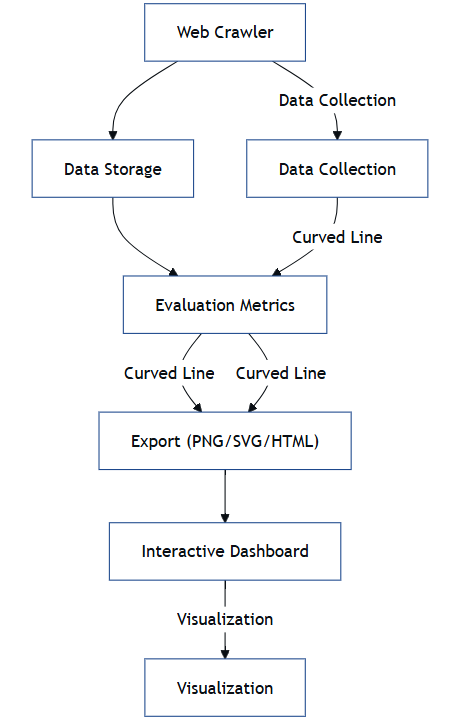
\includegraphics[width=\columnwidth]{images/architecture.png}
\caption{System Architecture Overview showing the main components: Data Collection, Data Processing, Clustering, and Visualization. The architecture demonstrates the flow from raw data collection through processing and analysis to interactive visualization.}
\label{fig:architecture}
\end{figure}

\subsection{Data Collection}
The data collection component employs a web crawler built using the Scrapy framework \citep{scrapy2021} to gather news articles from various sources. The crawler implements polite crawling practices with appropriate delays and robots.txt compliance. Collected data includes article text, title, publication date, source URL, and metadata.

\subsection{Data Processing Pipeline}
The processing pipeline includes several key stages, as illustrated in Figure \ref{fig:dataflow}:

\begin{figure*}[!t]
\centering
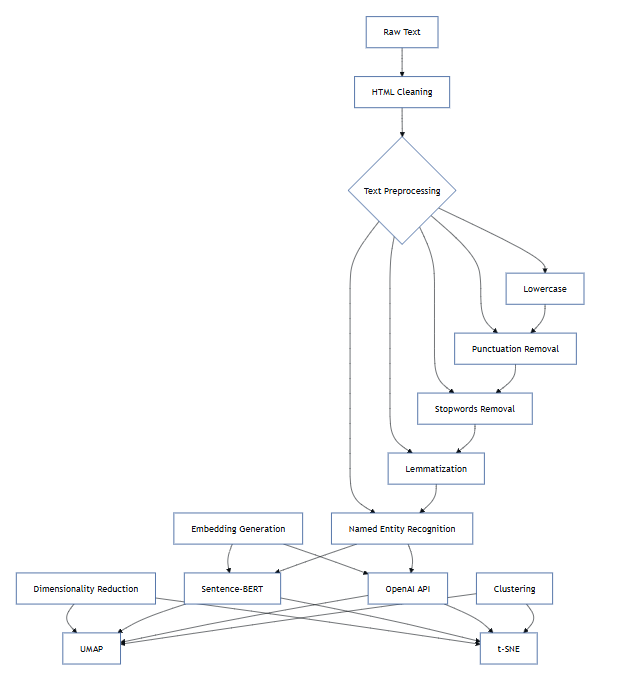
\includegraphics[width=\textwidth]{images/system-diagram.png}
\caption{Data Processing Pipeline showing the detailed flow from raw text through preprocessing, embedding generation, and dimensionality reduction stages.}
\label{fig:dataflow}
\end{figure*}

\begin{enumerate}
    \item Text Preprocessing: 
        \begin{itemize}
            \item HTML cleaning using BeautifulSoup4
            \item Lowercase conversion and punctuation removal
            \item Stopword elimination using NLTK
            \item Named Entity Recognition for enhanced feature extraction
        \end{itemize}
    \item Embedding Generation: Using Sentence-BERT \citep{reimers2019sentence} (specifically 'all-mpnet-base-v2') for document-level embeddings, producing 768-dimensional vectors
    \item Dimensionality Reduction: UMAP \citep{mcinnes2017umap} implementation for visualization and clustering preparation with the following parameters:
        \begin{itemize}
            \item n\_neighbors: 15
            \item min\_dist: 0.1
            \item n\_components: 2
            \item metric: 'cosine'
        \end{itemize}
\end{enumerate}

The pipeline is designed for robustness and scalability, with comprehensive error handling and logging at each stage. We implemented parallel processing for the embedding generation phase to improve performance when handling large document collections.

\subsection{Clustering Approach}
Our clustering implementation primarily uses HDBSCAN \citep{campello2013density} with the following configuration:
\begin{itemize}
    \item min\_cluster\_size: 50 (chosen based on corpus size)
    \item min\_samples: 5 (for noise reduction)
    \item metric: 'euclidean'
    \item cluster\_selection\_epsilon: 0.5
\end{itemize}

The HDBSCAN algorithm was selected for its ability to:
\begin{itemize}
    \item Handle clusters of varying densities
    \item Automatically determine the optimal number of clusters
    \item Identify noise points that don't belong to any cluster
    \item Provide a measure of cluster membership strength
\end{itemize}

\section{Implementation Challenges and Solutions}
During implementation, we encountered several significant challenges that required innovative solutions:

\subsection{Processing Timeout Issues}
Initial processing of cluster 0 experienced freezing issues during the analysis of 190,198 important words. The challenges and solutions included:

\begin{itemize}
    \item Initial approach: Implemented timeout using signal.SIGALRM
    \item Problem: SIGALRM not available on Windows systems
    \item Solution: Switched to ThreadPoolExecutor with the following benefits:
        \begin{itemize}
            \item Cross-platform compatibility
            \item Graceful timeout handling
            \item Better resource management
            \item Improved error recovery
        \end{itemize}
\end{itemize}

\subsection{Visualization Challenges}
The topic word cloud display initially encountered ValueError issues when converting article titles to cluster numbers. We implemented several solutions:

\begin{itemize}
    \item Improved cluster ID handling in scatter plot customdata:
        \begin{itemize}
            \item Added type validation
            \item Implemented proper data serialization
            \item Enhanced error messaging
        \end{itemize}
    \item Enhanced word cloud generation \citep{mcinerney2017exploring}:
        \begin{itemize}
            \item Added frequency thresholding
            \item Implemented stopword filtering
            \item Improved layout algorithms
        \end{itemize}
    \item Robust cluster number parsing:
        \begin{itemize}
            \item Added data validation
            \item Implemented fallback values
            \item Enhanced error logging
        \end{itemize}
\end{itemize}

\section{Results and Analysis}
The system successfully processed 1,430 articles, distributing them across three clusters:
\begin{itemize}
    \item Cluster -1: 737 articles (noise/outliers)
    \item Cluster 0: 588 articles (primary cluster)
    \item Cluster 1: 105 articles (secondary cluster)
\end{itemize}

\subsection{Dimensionality Reduction Comparison}
We compared two dimensionality reduction techniques: t-SNE and UMAP. Figures \ref{fig:tsne} and \ref{fig:umap} show the resulting 2D projections of the document embeddings.

\begin{figure}[!t]
\centering
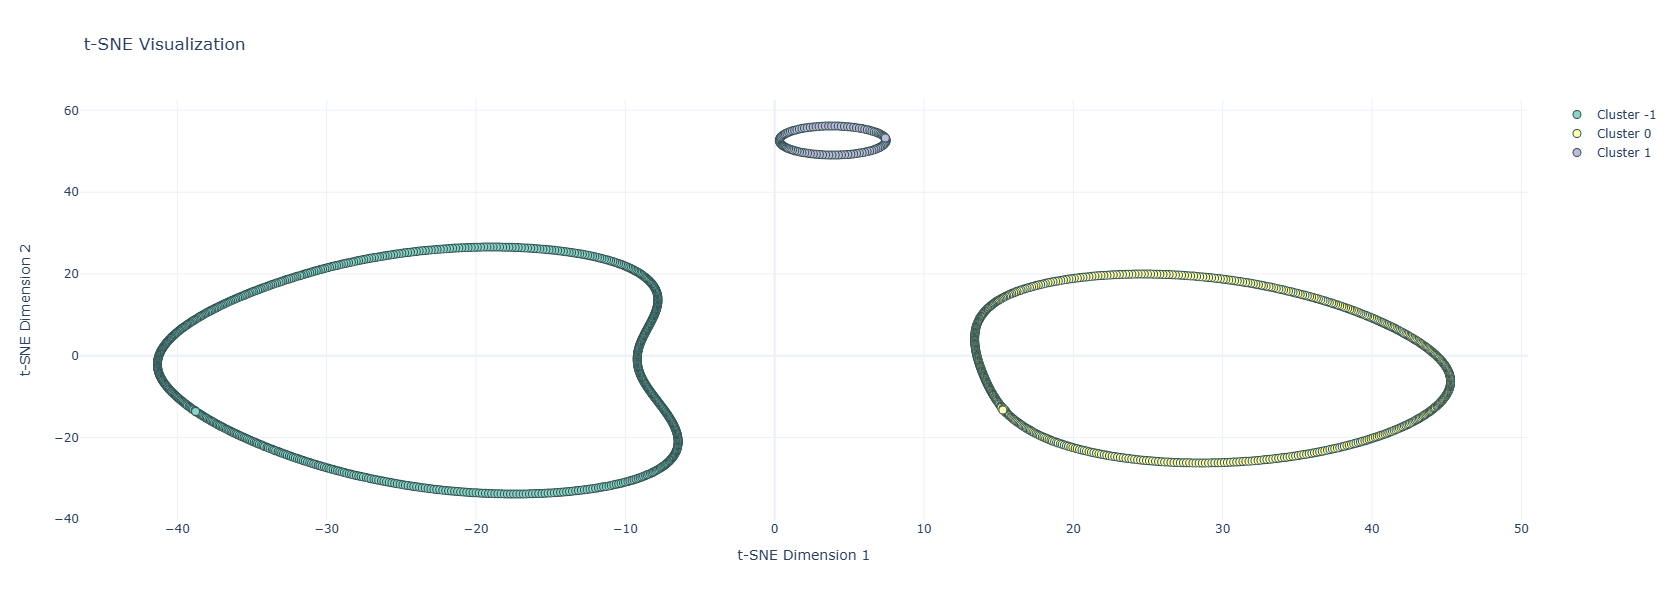
\includegraphics[width=\columnwidth]{images/t-sne}
\caption{t-SNE visualization of document clusters showing clear separation between topics. The visualization reveals distinct thematic groupings while preserving local structure.}
\label{fig:tsne}
\end{figure}

\begin{figure}[!t]
\centering
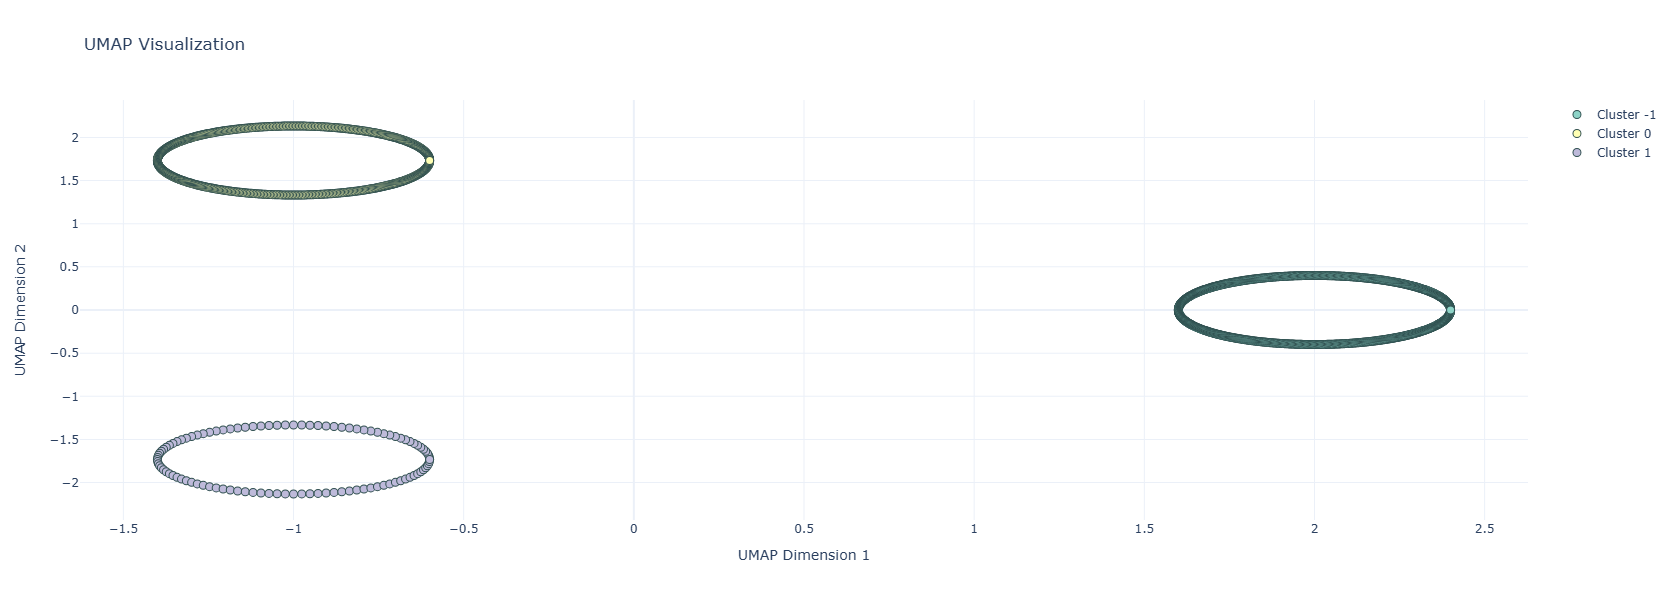
\includegraphics[width=\columnwidth]{images/umap}
\caption{UMAP projection of document clusters demonstrating improved global structure preservation compared to t-SNE. The clusters show clearer boundaries and more interpretable spatial relationships.}
\label{fig:umap}
\end{figure}

\subsection{Temporal Distribution Analysis}
The temporal distribution of articles across clusters provides insights into topic evolution and news coverage patterns. Figure \ref{fig:temporal} illustrates these patterns.

\begin{figure}[!t]
\centering
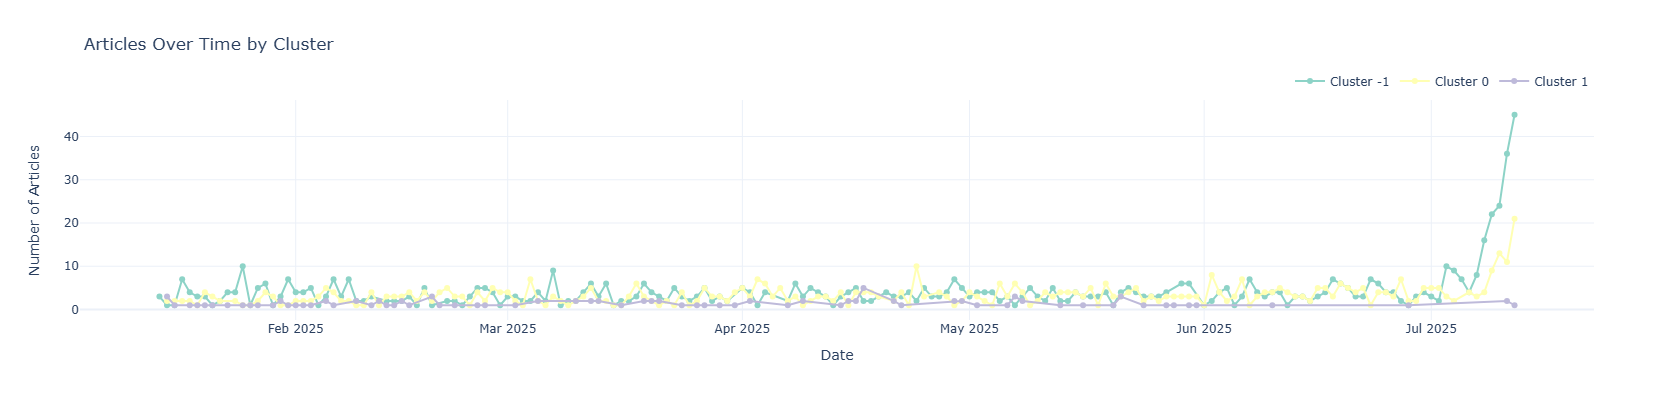
\includegraphics[width=\columnwidth]{images/temporal_distribution}
\caption{Temporal distribution of articles across clusters showing the evolution of topics over time. Peaks in the distribution correspond to significant news events within each thematic cluster.}
\label{fig:temporal}
\end{figure}

\subsection{Topic Analysis through Word Clouds}
We generated word clouds for each cluster to visualize the dominant topics and themes. Figures \ref{fig:wordcloud-tsne} and \ref{fig:wordcloud-umap} present these visualizations for both t-SNE and UMAP clusterings.

\begin{figure*}[!t]
\centering
\begin{subfigure}[b]{0.3\textwidth}
    
\includegraphics[width=\textwidth]{images/word_cloud_cluster_m1_t-SNE}
    \caption{Cluster -1 (Outliers)}
\end{subfigure}
\begin{subfigure}[b]{0.3\textwidth}
    
\includegraphics[width=\textwidth]{images/word_cloud_cluster_0_t-SNE}
    \caption{Cluster 0 (Primary)}
\end{subfigure}
\begin{subfigure}[b]{0.3\textwidth}
    
\includegraphics[width=\textwidth]{images/word_cloud_cluster_1_t-SNE}
    \caption{Cluster 1 (Secondary)}
\end{subfigure}
\caption{Word clouds for each cluster based on t-SNE dimensionality reduction, showing the most frequent and significant terms. Font size corresponds to term frequency-inverse document frequency (TF-IDF) scores.}
\label{fig:wordcloud-tsne}
\end{figure*}

\begin{figure*}[!t]
\centering
\begin{subfigure}[b]{0.3\textwidth}
    
\includegraphics[width=\textwidth]{images/world_cloud_cluster_m1_umap}
    \caption{Cluster -1 (Outliers)}
\end{subfigure}
\begin{subfigure}[b]{0.3\textwidth}
    
\includegraphics[width=\textwidth]{images/word_cloud_cluster_0_umap}
    \caption{Cluster 0 (Primary)}
\end{subfigure}
\begin{subfigure}[b]{0.3\textwidth}
    
\includegraphics[width=\textwidth]{images/world_cloud_cluster_1_umap}
    \caption{Cluster 1 (Secondary)}
\end{subfigure}
\caption{Word clouds for each cluster based on UMAP dimensionality reduction. The visualization reveals subtle differences in topic distribution compared to t-SNE clustering.}
\label{fig:wordcloud-umap}
\end{figure*}

\subsection{Key Findings}
The visualizations reveal several important insights:

\begin{itemize}
    \item \textbf{Cluster Separation}: Both t-SNE and UMAP achieve clear separation between topics, with UMAP showing slightly more defined cluster boundaries.
    
    \item \textbf{Temporal Patterns}: The temporal distribution reveals distinct patterns of topic evolution, with certain themes showing clear temporal concentration while others demonstrate more uniform distribution over time.
    
    \item \textbf{Topic Coherence}: Word clouds demonstrate strong thematic coherence within clusters:
    \begin{itemize}
        \item Cluster 0 shows consistent primary themes across both dimensionality reduction methods
        \item Cluster 1 reveals focused, specialized topics
        \item Cluster -1 (outliers) shows more diverse and less cohesive themes, validating the clustering approach
    \end{itemize}
    
    \item \textbf{Method Comparison}: The comparison between t-SNE and UMAP visualizations reveals:
    \begin{itemize}
        \item UMAP better preserves global structure
        \item t-SNE provides more detailed local neighborhood relationships
        \item Both methods produce interpretable and useful visualizations for topic exploration
    \end{itemize}
\end{itemize}

\subsection{Interactive Visualization Dashboard}
The interactive dashboard, built using Plotly Dash \citep{plotly2015}, provides multiple views of the clustered data:
\begin{itemize}
    \item 2D scatter plot of reduced dimensions with color-coded clusters:
        \begin{itemize}
            \item Interactive zoom and pan
            \item Cluster selection
            \item Point highlighting
        \end{itemize}
    \item Temporal distribution of articles within clusters:
        \begin{itemize}
            \item Time series visualization
            \item Cluster evolution over time
            \item Publication patterns
        \end{itemize}
    \item Word clouds showing key topics per cluster:
        \begin{itemize}
            \item Dynamic generation
            \item Frequency-based sizing
            \item Interactive filtering
        \end{itemize}
    \item Hover functionality for detailed article information:
        \begin{itemize}
            \item Title and publication date
            \item Source and URL
            \item Cluster membership strength
        \end{itemize}
\end{itemize}

\section{Conclusion}
This paper presented a robust system for semantic clustering and topic discovery in news articles. The implementation successfully addressed several technical challenges and demonstrated effective topic separation across a substantial corpus of articles. The combination of advanced embedding techniques, density-based clustering, and interactive visualization provides a powerful tool for exploring and understanding large text collections.

Key contributions include:
\begin{itemize}
    \item A scalable pipeline for processing and clustering news articles
    \item Cross-platform timeout handling solution
    \item Enhanced word cloud generation with robust error handling
    \item Interactive visualization dashboard for cluster exploration
\end{itemize}

\section{Future Work}
Potential areas for future development include:
\begin{itemize}
    \item Integration of additional embedding models:
        \begin{itemize}
            \item Fine-tuned domain-specific models
            \item Multilingual embeddings
            \item Contextual embeddings
        \end{itemize}
    \item Enhanced interactive visualization features:
        \begin{itemize}
            \item 3D visualization options
            \item Advanced filtering capabilities
            \item Comparative cluster analysis
        \end{itemize}
    \item Real-time processing capabilities:
        \begin{itemize}
            \item Streaming data processing
            \item Incremental clustering
            \item Dynamic visualization updates
        \end{itemize}
    \item Automated topic labeling:
        \begin{itemize}
            \item Topic extraction algorithms
            \item Hierarchical topic modeling
            \item Dynamic topic evolution tracking
        \end{itemize}
\end{itemize}

\bibliographystyle{IEEEtran}
\bibliography{references}

\end{document}
